% Курсовая работа. Компиляция: XeLaTeX + Biber (latexmk -xelatex main.tex).
\documentclass[14pt,a4paper,oneside]{extarticle}

% --- Кодировка, язык, шрифт (XeLaTeX) ---
\usepackage{fontspec}
\usepackage{polyglossia}
\setmainlanguage{russian}
\setotherlanguage{english}
\defaultfontfeatures{Ligatures=TeX}
\setmainfont{Times New Roman}
\setmonofont{Courier New}[Scale=MatchLowercase]
\newfontfamily\cyrillicfont{Times New Roman}
\newfontfamily\cyrillicfonttt{Courier New}[Scale=MatchLowercase]

% --- Геометрия страницы (левое поле >= 2 см; берём ГОСТ-поля) ---
\usepackage[a4paper,left=30mm,right=15mm,top=20mm,bottom=20mm]{geometry}

% --- Межстрочный интервал 1,5 и красная строка 1 см ---
\usepackage{setspace}
\onehalfspacing
\setlength{\parindent}{1cm}

% --- Аккуратная правая граница: микротипографика + аварийный растяг ---
\usepackage{microtype}
\setlength{\emergencystretch}{3em}

% --- Графика, таблицы, формулы ---
\usepackage{graphicx}
\graphicspath{{figures/}}
\usepackage{pdfpages}
\usepackage{tikz}
\usetikzlibrary{arrows.meta,positioning,shapes.geometric,fit,backgrounds}
\usepackage{placeins}
\usepackage{booktabs}
\usepackage{array}
\usepackage{longtable}
\usepackage{multirow}
\usepackage{amsmath}
\usepackage{amssymb}
\usepackage{siunitx}

% --- Подписи: рисунки снизу по центру (Рис. 2.3.), таблицы сверху справа (Таблица 2.3.) ---
\usepackage{caption}
\captionsetup{labelsep=period}
\captionsetup[figure]{name=Рис.,justification=centering,position=bottom}
\captionsetup[table]{name=Таблица,justification=raggedleft,singlelinecheck=false,position=top}

% --- Нумерация объектов внутри глав (через точку: 2.3) ---
\numberwithin{figure}{section}
\numberwithin{table}{section}
\numberwithin{equation}{section}

% --- Заголовки разделов ---
\usepackage{titlesec}
\titleformat{\section}{\normalfont\large\bfseries}{\thesection}{0.6em}{}
\titleformat{\subsection}{\normalfont\normalsize\bfseries}{\thesubsection}{0.6em}{}
\titleformat{\subsubsection}{\normalfont\normalsize\itshape}{\thesubsubsection}{0.6em}{}
\titlespacing*{\section}{0pt}{14pt}{8pt}
\titlespacing*{\subsection}{0pt}{12pt}{6pt}

% --- Содержание ---
\usepackage{tocloft}
\renewcommand{\cfttoctitlefont}{\hfill\large\bfseries}
\renewcommand{\cftaftertoctitle}{\hfill}

% --- Гиперссылки и перекрёстные ссылки ---
\usepackage[hidelinks,unicode]{hyperref}
\usepackage{xurl}

% --- Переносимый моноширинный код (рвётся по /, _, .) для длинных путей ---
\DeclareUrlCommand\code{\urlstyle{tt}}

% --- Библиография: ГОСТ Р 7.0.5-2008, числовой стиль ---
\usepackage[backend=biber,style=gost-numeric,sorting=none,language=auto,autolang=other]{biblatex}
\addbibresource{references.bib}

% --- Нумерация страниц: снизу по центру, на титуле не печатается ---
\pagestyle{plain}

\begin{document}

% Титульный лист (не нумеруется)
\IfFileExists{build/title_page.pdf}{%
  \includepdf[pages=1,pagecommand={\thispagestyle{empty}}]{build/title_page.pdf}%
}{%
  \begin{titlepage}
\thispagestyle{empty}
\begin{singlespace}
\newcommand{\titlepagefont}{\fontsize{13pt}{15.6pt}\selectfont}
\newcommand{\titlepagesmall}{\fontsize{11pt}{13.2pt}\selectfont}
\newcommand{\studentsignature}{%
  \IfFileExists{figures/student_signature.png}{%
    \raisebox{-0.25cm}{\includegraphics[height=0.85cm]{figures/student_signature.png}}%
  }{}%
}
\newcommand{\topicline}[3]{%
  \noindent\begin{minipage}[t]{\textwidth}
  {\titlepagefont #2\hspace{0.25cm}{\fontsize{12pt}{14.4pt}\selectfont #3}\par}
  \vspace{-0.16cm}
  \hspace*{#1}\rule{\dimexpr\textwidth-#1\relax}{0.4pt}
  \end{minipage}%
}
\centering

{\titlepagefont
Федеральное государственное автономное образовательное учреждение\\
высшего образования «Национальный исследовательский университет\\
«Высшая школа экономики»\par}

\vspace{0.9cm}
{\titlepagefont Факультет компьютерных наук\par}

\vspace{0.2cm}
{\titlepagefont Магистерская программа Машинное обучение в цифровом продукте\par}

\vspace{1.9cm}
{\titlepagefont КУРСОВАЯ РАБОТА\par}

\vspace{1.0cm}
\topicline{3.35cm}{На тему (рус)}{Система кластеризации научных статей}

\vspace{0.45cm}
\topicline{3.85cm}{На тему (англ.)}{Scientific article clustering system}

\vspace{1.4cm}

\begin{flushright}
\begin{minipage}{0.55\textwidth}
\raggedright
{\titlepagefont
Студент\\[0.35cm]
\makebox[7.6cm][l]{Белкин Андрей Александрович\hfill\studentsignature}\\[-0.28cm]
\rule{7.6cm}{0.4pt}\\[-0.05cm]
{\titlepagesmall\hspace*{1.65cm}(Ф.И.О., подпись)}\\[0.85cm]

Руководитель КР\\[0.35cm]
\makebox[7.6cm][l]{старший преподаватель А.\,А.~Паринов}\\[-0.05cm]
\rule{7.6cm}{0.4pt}\\[-0.05cm]
{\titlepagesmall (должность, звание, Ф.И.О, подпись)}
}
\end{minipage}
\end{flushright}

\vfill
{\titlepagefont Москва, 2026\par}

\end{singlespace}
\end{titlepage}
%
}

% Аннотации RU/EN (не нумеруются)
\thispagestyle{empty}
\section*{Аннотация}

В работе разработана и реализована система <<AI Coauthor>> — комплекс семантического
анализа научного пространства, тематической кластеризации публикаций и рекомендации
потенциальных научных соавторов с объяснениями на основе больших языковых моделей.
Цель работы — построить инструмент, который по тексту научных статей выявляет тематическую
структуру предметной области и обоснованно подсказывает исследователю семантически
совместимых коллег. Эмпирическую базу составляет корпус из 509\,447 публикаций OpenAlex
по подполю Artificial Intelligence и 35\,954 квалифицированных авторов. Статьи представлены
многоязычными эмбеддингами модели multilingual-e5-base (768 измерений); тематическая
структура из 979 тем получена пайплайном в стиле BERTopic (UMAP $\to$ HDBSCAN $\to$
c-TF-IDF $\to$ MMR $\to$ разметка языковой моделью), а 979 тем дополнительно объединены
в 76 метакластеров — семантический слой над темами. HDBSCAN сравнивался с наивными
бейзлайнами K-Means и случайным разбиением на UMAP-10; выбор обоснован по совокупности
независимых метрик качества тем. Рекомендация соавторов реализована в два этапа:
mean-, Transformer- и GraphSAGE-представления автора извлекают близких кандидатов (retrieval),
после чего пятиступенчатый пайплайн на основе языковой модели переранжирует их и формирует
объяснения с конкретными попарными связями статей. Качество финальной выдачи оценено
LLM-судьёй: LLM Has3@10 (score $\geq 2$) = 0,875, LLM Selected3Mean@10 = 2,49 из 3.
Результат интегрирован в
веб-приложение с интерактивной картой научного пространства.

\newpage
\thispagestyle{empty}
\section*{Abstract}

\begin{english}
This work presents AI Coauthor, a system for the semantic analysis of the scientific landscape:
it performs topic clustering of publications and recommends potential research collaborators with
explanations produced by large language models. The goal is a tool that recovers the topical
structure of a research field directly from paper texts and suggests semantically compatible peers
in a justified, interpretable way. The empirical base is a corpus of 509{,}447 OpenAlex publications
in the Artificial Intelligence subfield and 35{,}954 qualified authors. Papers are represented by
multilingual embeddings from the multilingual-e5-base model (768 dimensions); a topical structure
of 979 topics is obtained with a BERTopic-style pipeline (UMAP $\to$ HDBSCAN $\to$ c-TF-IDF
$\to$ MMR $\to$ LLM labeling), and the 979 topics are further grouped into 76 meta-clusters, a
semantic layer over the topics. HDBSCAN is compared against naive K-Means and random baselines on
UMAP-10; the choice is justified through a set of independent topic-quality metrics. Collaborator
recommendation is built in two stages: mean, Transformer, and GraphSAGE author representations retrieve nearby
candidates, after which a five-stage LLM pipeline re-ranks them and generates explanations grounded
in concrete pairwise paper links. The final recommendations are evaluated with an LLM judge:
LLM Has3@10 (score $\geq 2$) = 0.875, and LLM Selected3Mean@10 reaches 2.49 out of 3. The
result is integrated into a web application with an
interactive map of the scientific space.
\end{english}


% Содержание (титул и аннотации не нумеруются; сквозной номер начинается здесь)
\clearpage
\setcounter{page}{4}
\tableofcontents
\newpage

% Введение
\section*{Введение}
\addcontentsline{toc}{section}{Введение}

Объём научной литературы растёт экспоненциально: по разным оценкам число публикаций
удваивается примерно каждые 10–15 лет~\cite{bornmann2015growth}. На таком фоне исследователю
всё труднее удерживать в голове карту собственной области — отслеживать смежные направления,
видеть, где его работа граничит с чужой, и находить людей, с которыми имеет смысл начать
совместный проект. Классические библиометрические инструменты опираются прежде всего на графы
цитирований и соавторства~\cite{newman2001coauthorship}. Такие графы хорошо описывают уже
состоявшиеся связи, но почти не подсказывают новые: задача предсказания ещё не возникших рёбер
(link prediction) в социальных и научных сетях известна своей сложностью~\cite{libennowell2007link},
а главное — формальная связь <<кто кого процитировал>> слабо отражает смысловую близость работ.

Ситуация изменилась с приходом трансформерных архитектур. Сначала
BERT~\cite{devlin2019bert} показал, что предобученный энкодер хорошо улавливает контекст слова,
а затем энкодерные модели эмбеддингов вроде Sentence-BERT~\cite{reimers2019sbert} научились
кодировать смысл целого текста в один вектор так, что семантически близкие документы
оказываются рядом в пространстве. Это позволяет перейти от формальных связей к семантическому
анализу — представить статью вектором, сгруппировать корпус по смыслу, а не по совпадению
ключевых слов, и оценить близость двух исследователей по содержанию их работ, даже если в
списке соавторов они никогда не пересекались. Параллельно большие языковые
модели (LLM) дали возможность не только ранжировать кандидатов, но и объяснять рекомендацию на
естественном языке, а заодно выступать оценщиком качества (LLM-as-a-judge) там, где ручная
разметка слишком дорога~\cite{zheng2023judging}. Наконец, открытые базы вроде
OpenAlex~\cite{priem2022openalex} сделали корпус из сотен тысяч статей с метаданными доступным
без коммерческих ограничений.

\textbf{Тема работы} — система кластеризации научных статей.

\textbf{Объект исследования} — научное информационное пространство: корпус публикаций и
исследователи, стоящие за ними. \textbf{Предмет исследования} — методы векторного представления
статей, тематической кластеризации публикаций и поиска семантически совместимых соавторов с
генерацией объяснений.

Отдельно поясню постановку задачи рекомендаций — здесь легко допустить неточность.
Рекомендатель состоит из двух частей. Первая, обучаемая, — этап извлечения (retrieval):
нейросетевая модель по истории публикаций автора строит вектор его научных интересов, и мы
отбираем авторов с наиболее близкими векторами. То есть retrieval находит исследователей с
близкой тематической траекторией, а не «дополняющих» друг друга — это важно не путать. Вторая
часть — переранжирование на предобученной языковой модели: она оценивает релевантность
отобранных кандидатов и уже способна выделять взаимодополняющую экспертизу, формируя
объяснение. Обучается в системе только первая часть; языковая модель используется без
дообучения. Результат мы сознательно не называем «предсказанием будущего соавтора»: фактические
соавторства — разреженный и неполный сигнал, они покрывают лишь часть всех релевантных связей,
поэтому корректнее говорить об извлечении и ранжировании совместимых кандидатов (количественно
этот разрыв показан в главе~3).

\textbf{Цель работы} — разработать систему семантического анализа научного пространства, которая
строит векторные представления статей, выполняет интерпретируемую тематическую кластеризацию,
визуализирует пространство в виде интерактивной карты и рекомендует совместимых соавторов с
понятными объяснениями.

Для достижения цели поставлены следующие \textbf{задачи}:

\begin{enumerate}
  \item собрать корпус научных публикаций из OpenAlex и привести тексты к единому виду;
  \item построить многоязычные эмбеддинги статей;
  \item реализовать пайплайн тематической кластеризации в стиле BERTopic;
  \item сравнить HDBSCAN с наивными бейзлайнами (K-Means и случайное разбиение на UMAP-10)
        по набору независимых метрик и обоснованно выбрать лучший вариант;
  \item построить семантический слой метакластеров — укрупнённое объединение мелких тем в крупные
        группы;
  \item обучить нейросетевую модель представления автора и реализовать retrieval кандидатов;
  \item реализовать LLM-переранжирование кандидатов и генерацию объяснений;
  \item разработать веб-приложение с интерактивной картой и интерфейсом рекомендаций;
  \item провести эксперименты: оценить качество кластеризации, retrieval и рекомендаций.
\end{enumerate}

\textbf{Методы исследования.} Векторизация статей — multilingual-e5-base~\cite{wang2024multilinguale5};
понижение размерности — UMAP~\cite{mcinnes2018umap}; кластеризация — HDBSCAN~\cite{campello2013hdbscan,
mcinnes2017hdbscanjoss}; интерпретируемое представление тем — c-TF-IDF
и Maximal Marginal Relevance~\cite{carbonell1998mmr} в духе BERTopic~\cite{grootendorst2022bertopic};
представление автора — Transformer-энкодер~\cite{vaswani2017attention} и GraphSAGE
поверх графа соавторства~\cite{hamilton2017graphsage} с обучением по coauthor InfoNCE;
оценка качества — proxy-метрики по будущим соавторам, в том числе nDCG~\cite{jarvelin2002ndcg},
и LLM-as-a-judge~\cite{zheng2023judging} для релевантности финальной выдачи.

\textbf{Основной результат.} Реализована работающая система <<AI Coauthor>>. На корпусе из
509\,447 статей по подполю Artificial Intelligence и 35\,954 квалифицированных авторов построены
979 тем и 76 метакластеров. HDBSCAN выбран по совокупности метрик качества тем с явным
компромиссом по доле шума. Рекомендательный пайплайн
сравнен в трёх режимах — mean-бейзлайн, Transformer и GraphSAGE; LLM Has3@10 (score $\geq 2$)
равен 0,875, а LLM Selected3Mean@10 достигает 2,49 из 3. Графовый метод даёт
сопоставимое качество с Transformer, но не показывает значимого выигрыша от кластерных узлов. Все
подсистемы объединены в веб-приложение
с интерактивной картой научного пространства.

\textbf{Структура работы.} Работа состоит из введения, трёх глав, заключения и
библиографического списка. В главе~1 дан обзор предметной области: научные графы, текстовые
эмбеддинги, тематическое моделирование, рекомендация соавторов и подход LLM-as-a-judge. В
главе~2 описаны архитектура и реализация системы AI~Coauthor — от сбора данных и построения
эмбеддингов до кластеризации, метакластеров, рекомендательного пайплайна и веб-приложения. В
главе~3 приведены эксперименты: описание датасета, сравнение кластеризации с бейзлайнами,
retrieval-метрики и LLM-оценка качества рекомендаций. В заключении подведены итоги и обозначены
ограничения и направления развития.


% Главы
\newpage
\section{Обзор предметной области}
\label{ch:review}

Система кластеризации научных статей и построенный поверх неё рекомендатель соавторов стоят на
стыке нескольких областей: библиометрии и анализа научных графов, обработки естественного языка,
тематического моделирования и информационного поиска. Чтобы обосновать инженерные решения главы~2,
ниже разобраны пять блоков: источники данных и графовые методы, текстовые эмбеддинги, тематическое
моделирование, рекомендация научных соавторов и применение больших языковых моделей в роли
оценщика. В каждом блоке отмечено, почему «классический» подход в нашей задаче упирается в потолок,
и какой инструмент приходит ему на смену.

\subsection{Научные графы, источники данных и предсказание связей}

Исторически анализ науки строится на графах. Граф цитирований связывает работы по ссылкам, граф
соавторства — исследователей по совместным публикациям. Структуру таких сетей подробно изучил
Ньюман~\cite{newman2001coauthorship}: у большинства авторов соавторов немного, тогда как у
отдельных — очень много, и при этом почти все исследователи оказываются связаны в одну крупную
компоненту. Такие графы хорошо отвечают на вопрос «кто с кем уже связан», но для рекомендации
новых связей их приходится достраивать.

Сырьём для графов служат библиографические базы. Долгое время эталоном был Microsoft Academic
Graph~\cite{sinha2015mag}, однако после его закрытия открытым преемником стал
OpenAlex~\cite{priem2022openalex} — полностью открытый индекс работ, авторов, площадок и
организаций, который мы и используем как источник корпуса.

Задача рекомендации новой связи в графовой постановке — это \emph{предсказание связей} (link
prediction). Либен-Ноуэлл и Клейнберг~\cite{libennowell2007link} показали, что по одной лишь
топологии сети (общие соседи, мера Адамика–Адара и т.\,п.) будущие рёбра предсказываются заметно
лучше случайного, но точность остаётся невысокой. Главное ограничение для нас в другом: чисто
структурные признаки не видят \emph{смысла} работ. Два исследователя могут заниматься почти
одинаковыми задачами, но если в графе между ними нет коротких путей — топологический метод их не
сблизит. Отсюда вытекает потребность в содержательном, текстовом представлении публикаций.

Современные графовые нейросети ослабляют это ограничение: они агрегируют не только структуру
соседства, но и признаки узлов. В GraphSAGE~\cite{hamilton2017graphsage} представление узла
строится через сообщения от соседей и собственные признаки узла, поэтому метод можно применить к
графу соавторства, инициализировав авторов семантическими признаками по их статьям. Такая модель
не заменяет текстовые эмбеддинги, а проверяет, добавляет ли граф прошлых соавторств полезный сигнал
поверх семантического представления автора.

\subsection{Текстовые эмбеддинги}

Чтобы сравнивать статьи по смыслу, текст нужно превратить в вектор. Ранние подходы — мешок слов и
TF-IDF — игнорируют порядок и синонимию, а первые плотные представления слов
(word2vec~\cite{mikolov2013word2vec}) дали векторы для отдельных слов, но не для предложений и тем
более не учитывали контекст: слово получало один вектор на все смыслы.

Перелом принесли трансформерные модели. BERT~\cite{devlin2019bert} — предобученный двунаправленный
энкодер — научился строить \emph{контекстные} представления токенов, однако его выходы в исходном
виде плохо подходят для прямого сравнения текстов по косинусной близости. Эту проблему решил
Sentence-BERT~\cite{reimers2019sbert}: дообучение на парах предложений даёт эмбеддинги, которые уже
можно осмысленно сравнивать скалярным произведением. С тех пор стандартом стали специализированные
энкодеры предложений и документов.

Для нашего корпуса критична многоязычность — статьи OpenAlex написаны на разных языках. Поэтому
для векторизации статей выбрана модель multilingual-e5-base~\cite{wang2024multilinguale5}: она
строит единое векторное пространство для многих языков при префиксе \texttt{query:} и позволяет
кластеризовать и сравнивать работы независимо от языка оригинала. Косинусная близость таких
эмбеддингов служит рабочей мерой семантического сходства на этапах кластеризации и retrieval.
Для метадокументов метакластеров (короткие текстовые описания тем) используется та же
модель multilingual-e5-base с префиксом \texttt{query:}.

\subsection{Тематическое моделирование}

Группировка статей по темам — классическая задача. Долгое время её решало вероятностное
тематическое моделирование, прежде всего латентное размещение Дирихле
(LDA)~\cite{blei2003lda}: документ моделируется как смесь тем, тема — как распределение над словами.
LDA работает с мешком слов и потому плохо переносит короткие тексты (а аннотация — это короткий
текст) и не использует семантику эмбеддингов.

Современная альтернатива — embedding-based тематическое моделирование, канонический представитель
которого BERTopic~\cite{grootendorst2022bertopic}. Его конвейер: эмбеддинги $\to$ понижение
размерности $\to$ плотностная кластеризация $\to$ интерпретируемое представление тем. На шаге
понижения размерности применяется UMAP~\cite{mcinnes2018umap}, сохраняющий локальную структуру
многообразия лучше линейных методов; кластеризацию выполняет HDBSCAN~\cite{campello2013hdbscan,
mcinnes2017hdbscanjoss} — иерархический плотностный алгоритм, который не требует заранее задавать
число кластеров $K$, помечает разреженные точки как шум и устойчив к неравномерной плотности. Это
важные свойства: число тем в корпусе заранее неизвестно, а «фоновые» статьи честнее пометить шумом,
чем приписывать к ближайшей теме силой.

Представление темы словами строится через \emph{class-based} TF-IDF (c-TF-IDF): кластер
рассматривается как один большой документ, и вес слова показывает его специфичность для темы в
целом. Чтобы итоговый список ключевых слов не состоял из синонимов, применяется Maximal Marginal
Relevance~\cite{carbonell1998mmr}, балансирующий релевантность и новизну отбираемых терминов.

Для честного сравнения с плотностным подходом в главе~3 добавлены наивные бейзлайны: случайное
разбиение и K-Means на том же пространстве UMAP-10 с тем же числом кластеров $K$. Они показывают,
насколько выигрыш HDBSCAN по LLM-когерентности и различимости оправдан относительно геометрически
простого разбиения.

\subsection{Рекомендация научных соавторов}

Рекомендация работ и соавторов — отдельное направление; обзор Бееля и
соавторов~\cite{beel2016survey} систематизирует подходы к рекомендации научных публикаций.
Условно методы делятся на два семейства. \emph{Графовые} (по сути — то же предсказание связей)
опираются на структуру сети соавторства и страдают теми же ограничениями: холодный старт и
слепота к смыслу. \emph{Контентные} сравнивают исследователей по текстам их работ — и именно сюда
ложатся эмбеддинги.

С масштабом корпуса прямое попарное сравнение становится дорогим, поэтому в информационном поиске
закрепилась двухэтапная схема \emph{retrieve-then-rerank}. На первом этапе быстрый плотный поиск
(dense retrieval) по близости векторов отбирает небольшой набор кандидатов; парадигму плотного
поиска для открытых вопросов формализовали Карпухин и соавторы в DPR~\cite{karpukhin2020dpr}. На
втором этапе кандидаты переранжируются более дорогой и точной моделью.

Чтобы получить вектор \emph{автора}, а не отдельной статьи, историю его публикаций нужно
агрегировать. Естественный инструмент — трансформерный энкодер~\cite{vaswani2017attention}: он
обрабатывает последовательность эмбеддингов статей автора и через механизм внимания сводит её в
единое представление. Такой обучаемый агрегатор и образует первый, retrieval-этап нашего
рекомендателя. Второй проверяемый вариант — GraphSAGE поверх графа соавторства: он использует
те же семантические признаки авторов, но дополнительно передаёт информацию по рёбрам прошлых
совместных публикаций.

\subsection{Большие языковые модели в роли оценщика}

Появление больших языковых моделей (LLM), способных к обучению по нескольким примерам и следованию
инструкциям~\cite{brown2020gpt3}, изменило не только генерацию текста, но и способ оценки. Там, где
ручная разметка релевантности слишком дорога, всё чаще применяют подход \emph{LLM-as-a-judge}:
языковая модель оценивает качество ответов по заданной шкале. Чжэн и соавторы~\cite{zheng2023judging}
показали, что такие оценки сильно коррелируют с человеческими, и одновременно описали характерные
смещения (позиционное, в пользу многословия), которые приходится контролировать продуманным
промптом и перемешиванием порядка кандидатов.

В нашей задаче LLM используется в трёх ролях: разметка тем человекочитаемыми названиями, оценка
релевантности пар «автор\,--\,кандидат» на этапе переранжирования и генерация объяснений
рекомендаций. Подход LLM-as-a-judge при этом служит и инструментом \emph{измерения} качества там,
где фактические соавторства дают слишком разреженный и заниженный сигнал (см. главу~3).

\subsection{Выводы и результаты по главе}

Обзор показывает логику дальнейших решений. Графовые методы хорошо описывают уже состоявшиеся
связи, но плохо подсказывают новые и не видят смысла работ, поэтому в основу системы кладутся
многоязычные эмбеддинги multilingual-e5-base. Для интерпретируемой тематической структуры выбран
embedding-based подход в стиле BERTopic с плотностной кластеризацией HDBSCAN; качество
сопоставляется с наивными бейзлайнами K-Means и случайного разбиения. Рекомендация соавторов
строится по схеме retrieve-then-rerank: mean-бейзлайн, обучаемый трансформерный агрегатор и
GraphSAGE-агрегатор графа соавторства извлекают кандидатов, а большая языковая модель выполняет
переранжирование и объяснение. Наконец, подход
LLM-as-a-judge выбран как способ честно измерить качество рекомендаций в условиях разреженного
целевого сигнала. Эти выборы и реализуются в главе~2.

\newpage
\section{Архитектура и реализация системы}
\label{ch:impl}

В этой главе описано, как обзорные решения главы~1 превращаются в работающую систему. Изложение
идёт по ходу данных: от сбора корпуса и построения эмбеддингов через кластеризацию и метакластеры
к рекомендательному пайплайну и веб-приложению. Сравнительные эксперименты, обосновывающие выбор
конкретных алгоритмов и значений гиперпараметров, вынесены в главу~3 — здесь приводятся уже
выбранные варианты.

\subsection{Общая архитектура}
\label{sec:arch}

Система построена как последовательность независимых этапов обработки данных и логически делится
на две фазы (рис.~\ref{fig:arch}). \textbf{Предподсчёт и обучение} выполняются заранее, офлайн:
корпус OpenAlex кодируется эмбеддингами, понижается по размерности, кластеризуется, темы получают
интерпретируемое представление и объединяются в метакластеры; параллельно по истории публикаций
обучается модель представления автора, и для всех авторов заранее вычисляются эмбеддинги.
\textbf{Инференс} происходит онлайн, в ответ на запрос: по выбранному автору быстро извлекаются
кандидаты, языковая модель их оценивает, отбирает, ищет доказательства и формирует объяснение.
Разделение существенно по нагрузке — тяжёлые вычисления (эмбеддинги, кластеризация, обучение)
делаются один раз, а на запрос пользователя приходится лишь лёгкий retrieval и несколько вызовов
языковой модели.

\begin{figure}[ht]
\centering
\resizebox{\textwidth}{!}{%
\begin{tikzpicture}[
  >={Stealth[round]},
  font=\scriptsize,
  box/.style={rectangle, rounded corners, draw=black!55, align=center,
              minimum height=8mm, inner sep=2.5pt, fill=blue!5},
  data/.style={box, fill=black!7},
  arr/.style={->, draw=black!65, thick}
]
% --- Предподсчёт ---
\node[data] (n1) at (0,0)      {OpenAlex\\(AI-корпус)};
\node[box]  (n2) at (3.1,0)    {Эмбеддинги\\e5-base};
\node[box]  (n3) at (6.3,0)    {UMAP 10D\\+ HDBSCAN};
\node[box]  (n4) at (9.6,0)    {c-TF-IDF, MMR,\\LLM-метки};
\node[box]  (n5) at (12.8,0)   {Метакластеры\\(HDBSCAN)};
\node[data] (n6) at (3.1,-1.8) {История\\авторов};
\node[box]  (n7) at (6.3,-1.8) {Transformer /\\GraphSAGE};
\node[box]  (n8) at (9.6,-1.8) {Эмбеддинги\\авторов};
\draw[arr] (n1)--(n2); \draw[arr] (n2)--(n3); \draw[arr] (n3)--(n4); \draw[arr] (n4)--(n5);
\draw[arr] (n6)--(n7); \draw[arr] (n7)--(n8);
\draw[arr] (n2)--(n6);
\begin{scope}[on background layer]
\node[draw=black!40, dashed, rounded corners, fill=black!3, inner sep=8pt,
      fit=(n1)(n5)(n6)(n8),
      label={[anchor=north west, font=\scriptsize\itshape]north west:Предподсчёт и обучение}] (offline) {};
\end{scope}
% --- Инференс ---
\node[data] (m1) at (0,-4.7)    {Запрос\\автора};
\node[box]  (m2) at (3.1,-4.7)  {Dense\\retrieval};
\node[box]  (m3) at (6.3,-4.7)  {LLM-оценка\\и отбор};
\node[box]  (m4) at (9.6,-4.7)  {Доказательства\\и объяснение};
\node[box]  (m5) at (12.8,-4.7) {Веб-\\интерфейс};
\draw[arr] (m1)--(m2); \draw[arr] (m2)--(m3); \draw[arr] (m3)--(m4); \draw[arr] (m4)--(m5);
\begin{scope}[on background layer]
\node[draw=black!40, dashed, rounded corners, fill=green!4, inner sep=8pt,
      fit=(m1)(m5),
      label={[anchor=north west, font=\scriptsize\itshape]north west:Инференс}] (online) {};
\end{scope}
\draw[arr, dashed] (offline.south) -- node[right, font=\scriptsize]{артефакты предподсчёта} (online.north);
\end{tikzpicture}%
}
\caption{Архитектура системы: фаза предподсчёта и обучения (офлайн) и фаза инференса (онлайн)}
\label{fig:arch}
\end{figure}

Переиспользуемый код вынесен в пакет \code{src/}, разбитый по доменам (сбор данных, эмбеддинги,
кластеризация, метакластеры, рекомендации, оценка, веб); запускаемые сценарии — тонкие обёртки в
\code{scripts/run_*.py}, а гиперпараметры зафиксированы в \code{configs/*.yaml}.

\paragraph{Воспроизводимость.} Результаты системы детерминированы. Эмбеддинги статей вычисляются
один раз и далее переиспользуются; все источники случайности зафиксированы единым сидом
($\mathrm{seed} = 42$ для UMAP, K-Means и обучения модели, тогда как HDBSCAN детерминирован при
фиксированном входе); температура языковой модели выставлена в $0$. При неизменных входных данных
и коде повторный запуск даёт тот же результат.

\paragraph{Технологический стек.} Выбор инструментов подчинён задаче, и каждый пункт обоснован:

\begin{itemize}
  \item \textbf{Эмбеддинги статей} — multilingual-e5-base: многоязычный корпус и быстрый локальный
        инференс на 509\,447 статей;
  \item \textbf{Понижение размерности} — UMAP: сохраняет локальную структуру многообразия лучше
        линейных методов;
  \item \textbf{Кластеризация} — HDBSCAN: не требует заранее задавать число тем и умеет выделять
        шум;
  \item \textbf{Представление автора} — Transformer-энкодер и GraphSAGE (PyTorch): агрегируют
        историю публикаций и граф прошлых соавторств;
  \item \textbf{Языковая модель} — OpenAI gpt-4.1-mini: разметка тем, оценка релевантности и
        генерация объяснений;
  \item \textbf{Backend} — FastAPI; \textbf{frontend} — Deck.gl: отрисовка сотен тысяч точек
        карты в браузере.
\end{itemize}

\subsection{Построение эмбеддингов статей}
\label{sec:emb}

Каждая статья превращается в один вектор, отражающий её смысл. На вход берётся заголовок и
аннотация; к ним добавляется префикс \texttt{query:}, требуемый моделью
multilingual-e5-base~\cite{wang2024multilinguale5}. Единый префикс для всех статей гарантирует,
что эмбеддинги получены в одном режиме и сравнимы между собой.

Текст токенизируется с ограничением $\mathrm{max\_length} = 512$ токенов и кодируется моделью
\code{intfloat/multilingual-e5-base}; вектор L2-нормализуется — тогда его скалярное произведение
с другим вектором равно косинусной близости.

Корпус — 509\,447 статей OpenAlex по подполю Artificial Intelligence; полный набор фильтров
отбора описан в разделе~3.1. Результат этапа — матрица эмбеддингов \code{embeddings.npy}
размера $(509\,447, 768)$ и список идентификаторов \code{paper_ids.json}. Список задаёт канонический
порядок статей: по нему все последующие этапы сопоставляют строку матрицы с конкретной статьёй.

\subsection{Кластеризация научных публикаций}
\label{sec:cluster}

Тематическая структура строится конвейером в стиле BERTopic: эмбеддинги $\to$ UMAP $\to$ HDBSCAN
$\to$ c-TF-IDF $\to$ MMR $\to$ разметка языковой моделью. UMAP понижает размерность с 768 до
10 измерений, сохраняя локальную структуру, после чего HDBSCAN выделяет плотные
тематические сгустки, не требуя заранее задавать число тем и помечая разреженные статьи как шум.

Каждая тема описывается набором характерных слов. Сначала по кластерам считается c-TF-IDF (кластер
рассматривается как один большой документ), затем MMR отбирает из топ-слов разнообразный, не
дублирующий сам себя набор терминов. Наконец, языковая модель получает эти термины и заголовки
представительных статей и возвращает короткое человекочитаемое название темы. Примеры получившихся
названий fine-тем: \emph{Memory-Enabled AI Chatbots for Personalized Support},
\emph{Physics-Informed Neural Networks for PDE Inference},
\emph{Deep Learning for Solar Irradiance Forecasting},
\emph{Human-Guided Reinforcement Learning in Robotics}.

Качество вариантов оценивается набором \emph{независимых} метрик (без сводного взвешенного балла):

\begin{itemize}
  \item \emph{когерентность} $c$ — насколько статьи внутри темы относятся к одному
        исследовательскому направлению; оценивается языковой моделью по шкале 0–3 и взвешивается
        по размеру темы; в сравнительных таблицах нормируется к $[0,1]$ делением на 3;
  \item \emph{различимость} $d$ — доля пар тем, которые языковая модель сочла дублирующими; чем
        меньше, тем лучше разделены темы;
  \item \emph{сбалансированность размеров} — отсутствие «мегатем», поглощающих корпус;
        измеряется по доле статей, приходящейся на пять крупнейших кластеров (top5, меньше — лучше);
  \item \emph{доля шума} $n$ — доля статей, не отнесённых ни к одной плотной теме (свойственна
        только HDBSCAN);
  \item \emph{энтропия назначений} $e$ — для мягких методов (приписывают статью нескольким темам
        с вероятностями) высокая энтропия означает размытые границы тем.
\end{itemize}

По совокупности этих метрик выбран вариант \texttt{hdbscan\_fine} с \textbf{979} темами
($\mathrm{min\_cluster\_size} = 10$, $\mathrm{min\_samples} = 5$, метод отбора кластеров — leaf):
он даёт наибольшую когерентность ($c = 2{,}80$, нормированная $\hat{c} = 0{,}93$) при приемлемой
различимости ($d = 0{,}11$). Цена выбора — высокая доля шума ($n = 0{,}65$): значительная часть
статей не попадает в плотные кластеры, что ожидаемо для неоднородного AI-корпуса; тем не менее
детализация и интерпретируемость fine-слоя важнее для карты. Сравнительные таблицы, бейзлайны
и обоснование выбора приведены в разделе~3.2.

\subsection{Метакластеры}
\label{sec:meta}

979 fine-тем — слишком детально для обзора предметной области целиком, поэтому темы дополнительно
объединяются в \textbf{76} метакластеров. Это \emph{семантическое} объединение, а не геометрическая
иерархия: каждая тема представляется метадокументом (её LLM-название, топ-термины c-TF-IDF и
заголовки представительных статей), метадокумент кодируется тем же эмбеддером
multilingual-e5-base, и уже эти эмбеддинги тем кластеризуются HDBSCAN.

Когерентность и различимость метакластеров оценены полноценной LLM-оценкой с отдельными
промптами для мета-уровня (судья оценивает, образуют ли fine-темы одну \emph{широкую}
исследовательскую область, а не узкую fine-тему). По когерентности лучшим оказался вариант
\texttt{meta\_hdbscan\_medium} ($K = 76$): $\hat{c} = 0{,}90$ ($c = 2{,}71$), доля дублирующих пар
$0\,\%$. На этом уровне HDBSCAN помечает около $11\,\%$ тем как разреженные; такие темы
присоединяются к ближайшему по вероятности метакластеру, так что все 979 тем в итоге распределены
по 76 группам. Полная сравнительная таблица — в разделе~3.2.

При $K = 76$ каждая группа объединяет в среднем $\approx 13$ fine-тем; подпись метакластера
наследует LLM-название доминирующей темы в группе и поэтому звучит как конкретное поднаправление
AI, а не как абстрактная метка верхнего уровня. Примеры названий метакластеров:
\emph{Evolutionary Algorithms and Optimization Methods},
\emph{Quantum Computing with Superconducting Circuits},
\emph{Deep Learning for Medical Image Analysis},
\emph{Interpretable and Explainable NLP Models}.

Метакластеры — это крупный смысловой слой над темами, но \textbf{не} области на карте, и причина
техническая. Метакластеры получены кластеризацией кластеров, то есть статьи и темы живут в разных
векторных пространствах. Двумерная UMAP-проекция способна хорошо разделить либо статьи, либо темы,
но не то и другое сразу; наша карта построена так, чтобы разделять \emph{статьи}, и области
метакластеров на ней неизбежно накладываются друг на друга. Поэтому метакластеры используются как
подписи и контекст, а от их геометрической отрисовки на карте сознательно отказались.

\subsection{Рекомендательная система: представление автора и извлечение кандидатов}
\label{sec:retrieval}

Рекомендатель состоит из обучаемого этапа извлечения (этот раздел) и этапа переранжирования
языковой моделью (раздел~\ref{sec:rerank}). Обучается только первый.

\paragraph{Представления автора.} В работе сравниваются три способа получить вектор автора.
Первый — \code{mean_author_embedding}: L2-нормализованное среднее эмбеддингов последних статей
до cutoff. Это простой и сильный semantic baseline без обучения. Второй — Transformer-retriever
(\code{recommendation/model.py}): он получает последовательность эмбеддингов статей автора,
упорядоченных по времени; в cluster-aware вариантах к каждой статье дополнительно присоединяется
soft membership $q$ по темам. Базовый вариант без кластеров использует $q$ нулевой размерности,
fine-вариант использует $q = 980$ (979 fine-кластеров + шум), meta-вариант агрегирует эти признаки
до 76 метакластеров + шум.

В Transformer-retriever каждая статья проецируется в скрытое пространство
$d_{\text{model}} = 256$. Чтобы модель учитывала темп публикаций, разрыв во времени между соседними
статьями (в годах) разбивается на интервалы 0, 1, 2, 3 и 4+ лет, и каждому интервалу сопоставлен
обучаемый вектор-добавка к представлению статьи. К последовательности добавляется специальный
обучаемый токен автора (по аналогии с \texttt{[CLS]}), чьё выходное представление
$h_{\mathrm{author}}$ агрегирует историю.

Предсказанный вектор интересов автора $\hat{e}$ живёт в том же пространстве, что и эмбеддинги
статей, потому что retrieval сравнивает авторов по косинусной близости их векторов. Модель строит
$\hat{e}$ как \emph{остаток} поверх среднего эмбеддинга истории:
\begin{equation}
\label{eq:author-emb}
\hat{e} = \mathrm{normalize}\!\left(\bar{h} + \alpha \cdot \mathrm{MLP}(h_{\mathrm{author}})\right),
\end{equation}
где $\bar{h}$ — среднее эмбеддингов статей автора, $\mathrm{MLP}$ — двухслойная голова с GELU,
$\alpha$ — обучаемый масштаб остатка, инициализированный нулём. При $\alpha = 0$ модель совпадает
с mean-бейзлайном (среднее эмбеддингов истории); обучение добавляет лишь полезное отклонение от
него. Такой якорь важен: mean-бейзлайн напрямую использует качественные paper embeddings, и без
остаточной схемы обучаемый retriever проигрывал ему.

\paragraph{Графовый вариант.} Третий способ — GraphSAGE-retriever
(\code{recommendation/graph_retrieval.py}). Узлы графа — 35\,954 квалифицированных автора, ребро
между авторами проводится, если они имели совместную публикацию до cutoff 2024. В графе
464\,752 направленных author-author ребра; веса построчно нормируются, повторные старые
коллаборации не увеличивают вес ребра. Начальный признак узла $x_v$ — L2-нормализованное среднее
эмбеддингов последних статей автора, то есть тот же сигнал, что в mean-бейзлайне.

Один слой GraphSAGE вычисляет сообщения отдельно по типам рёбер:
\begin{equation}
\label{eq:graphsage-layer}
h_v^{(\ell+1)} =
\operatorname{LayerNorm}\!\left(
W_0 h_v^{(\ell)} +
\sum_{r \in \mathcal{R}} W_r
\sum_{u \in \mathcal{N}_r(v)} w_{vu}^{(r)} h_u^{(\ell)}
\right),
\end{equation}
где $h_v^{(0)} = x_v$, $\mathcal{R}$ — типы отношений, $\mathcal{N}_r(v)$ — соседи узла $v$ по
отношению $r$, $w_{vu}^{(r)}$ — нормированный вес ребра. В реализованной модели два слоя
($L = 2$), скрытая размерность 256, dropout 0.2. Выход снова строится как остаток поверх исходного
семантического признака:
\begin{equation}
\label{eq:graphsage-out}
z_v = \operatorname{normalize}\!\left(x_v + \beta W_{\mathrm{out}} h_v^{(L)}\right).
\end{equation}

Вариант с метакластерами не разрезает граф на независимые подграфы. Это один гетерогенный граф:
к авторским узлам добавлены 76 узлов метакластеров и отношения author-meta / meta-author. Связь
автора с метакластером имеет вес по суммарной массе его статей в метакластере; сохраняются веса
$\geq 0{,}02$, а при отсутствии таких весов берётся самый вероятный метакластер. В этом варианте
добавляется 172\,376 направленных author-meta/meta-author рёбер. Он проверяет, помогают ли
метакластеры как смысловые hub-узлы в графовом retrieval.

\paragraph{Обучение.} Модель обучается multi-positive \textbf{coauthor InfoNCE} на косинусной
близости. Для примера $i$ с предсказанным вектором $\hat{e}_i$ и множеством позитивов
$\mathcal{P}_i$ (будущие квалифицированные соавторы, не встречавшиеся в истории до cutoff) потеря
равна
\begin{equation}
\label{eq:loss}
\mathcal{L}_i = -\log \frac{\sum_{j \in \mathcal{P}_i} \exp\!\bigl(\cos(\hat{e}_i,\, e_j)/\tau\bigr)}
{\sum_{k \in \mathcal{N}_i} \exp\!\bigl(\cos(\hat{e}_i,\, e_k)/\tau\bigr)},
\end{equation}
где $e_j$ — эмбеддинг соавтора в том же варианте модели, $\mathcal{N}_i$ — сэмплированные
негативы из пула авторов, позитивы исключены из знаменателя (не конкурируют как negatives),
$\tau = 0{,}05$ — температура. Обе обучаемые семьи используют AdamW и early stopping по
val nDCG@50. Для Transformer задано $\mathrm{lr} = 2\cdot10^{-4}$ и
$\mathrm{weight\_decay} = 0{,}05$; для GraphSAGE — $\mathrm{lr} = 10^{-3}$ и
$\mathrm{weight\_decay} = 10^{-2}$. У Transformer скорость обучения линейно растёт первые 10\,\%
шагов, затем плавно снижается по косинусу.

Качество на обучении дополнительно контролируется метрикой nDCG@10 на валидации, где правильным
ответом считается фактически наблюдавшееся последующее соавторство (рис.~\ref{fig:ndcg}). Абсолютные
значения малы — это прямое следствие разреженности целевого сигнала, которая разбирается в
разделе~3.3.

\begin{figure}[ht]
\centering
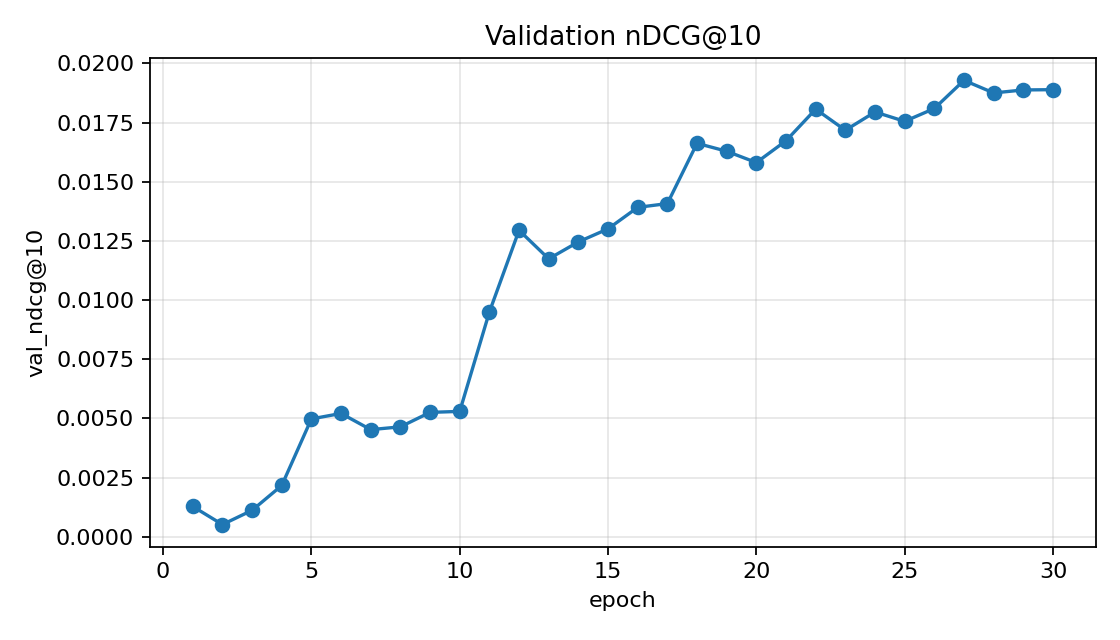
\includegraphics[width=0.78\textwidth]{val_ndcg10.png}
\caption{Валидационная метрика nDCG@10 Transformer-представления автора по эпохам обучения}
\label{fig:ndcg}
\end{figure}

\paragraph{Извлечение кандидатов (dense retrieval).} После обучения для каждого
квалифицированного автора (всего их \textbf{35\,954} — тех, у кого $\geq 10$ статей) предсказывается
вектор интересов. Эти векторы L2-нормализуются; для запрошенного автора вычисляется косинусная
близость со всеми остальными, исключаются он сам и его существующие соавторы (рекомендуем
\emph{новые} связи), и берутся топ-$N$ ближайших (в основной схеме $N = 10$). Это и есть кандидаты для
переранжирования. Подчеркну: на этом этапе отбираются именно ближайшие по вектору исследователи —
с похожей тематической траекторией; содержательная оценка релевантности выполняется уже на
следующем этапе.

\subsection{Переранжирование и генерация объяснений на основе языковой модели}
\label{sec:rerank}

Dense retrieval даёт быстрый, но грубый список — он не учитывает содержательные детали. Эту работу
выполняет пятиступенчатый пайплайн на языковой модели \texttt{gpt-4.1-mini} (рис.~\ref{fig:arch},
фаза инференса).

\begin{enumerate}
  \item \textbf{Retrieval.} Топ-$N$ кандидатов из раздела~\ref{sec:retrieval}.
  \item \textbf{Оценка релевантности.} Каждый кандидат оценивается отдельным вызовом языковой
        модели по шкале 0–3 (см. ниже): в промпт подаются недавние статьи автора и кандидата.
        Вызовы независимы и выполняются параллельно.
  \item \textbf{Отбор.} Берутся топ-$K$ кандидатов (по умолчанию $K = 3$) по оценке.
  \item \textbf{Извлечение доказательств.} Для каждого отобранного кандидата модель находит не
        более двух сильнейших попарных связей «статья автора\,$\leftrightarrow$\,статья кандидата»,
        возвращая индексы связываемых статей (только из переданных в промпт), краткую конкретную
        причину и ссылки OpenAlex.
  \item \textbf{Объяснение.} Модель формирует связный текст рекомендаций, ссылаясь только на
        реально переданные статьи — выдумывать их запрещено.
\end{enumerate}

Шкала релевантности: \textbf{0} — нерелевантно; \textbf{1} — слабое/общее совпадение (только широкая
близость в духе «оба про AI»); \textbf{2} — релевантно (конкретная общая задача, метод, тип данных
или взаимодополняющая экспертиза); \textbf{3} — очень релевантно (сильное конкретное совпадение).
Каждому кандидату присваивается \emph{тип связи}: прямое тематическое совпадение, совпадение по
методу, взаимодополняющая экспертиза или слабое/общее совпадение.

Ключевое требование к качеству — опираться на \emph{конкретные} связи, а не на общие фразы. В
промптах прямо запрещены обоснования вида «both papers discuss AI methodologies»; действует правило
\emph{«если связь сводится лишь к широкой близости по AI/ML — не включать её»}. Кандидаты с типом
«слабое/общее совпадение» отфильтровываются из финального списка. Именно здесь, в отличие от
retrieval, система способна различать взаимодополняющую экспертизу — это делает суждение языковой
модели, а не близость векторов.

\subsection{Веб-приложение}
\label{sec:web}

Все этапы сведены в веб-приложение: backend на FastAPI раздаёт статику и JSON-API, frontend на
ванильном JavaScript и Deck.gl отрисовывает сотни тысяч точек. Основные маршруты API перечислены
в таблице~\ref{tab:api}.

\begin{table}[ht]
\caption{Основные маршруты API backend}
\label{tab:api}
\centering
\footnotesize
\begin{tabular}{ll}
\toprule
Маршрут & Назначение \\
\midrule
\texttt{GET /api/map/state} & Точки статей, центры и подписи тем и метакластеров \\
\texttt{GET /api/papers/\{id\}} & Детали статьи \\
\texttt{GET /api/clusters/info/\{id\}} & Сводка по теме или метакластеру \\
\texttt{GET /api/authors/search} & Автодополнение поиска авторов \\
\texttt{POST /api/recommendations/\{id\}} & Запуск пайплайна рекомендаций \\
\bottomrule
\end{tabular}
\end{table}

Главный экран — карта научного пространства, где каждая точка это статья, окрашенная по своей теме
(рис.~\ref{fig:map}). Навигация построена на зуме: на дальнем масштабе видны крупные подписи
метакластеров, на среднем проявляются названия тем, на глубоком — заголовки отдельных статей.
Подписи плавно проявляются и затухают по уровню зума, а их пересечения устраняются встроенной
коллизионной фильтрацией Deck.gl.

\begin{figure}[ht]
\centering
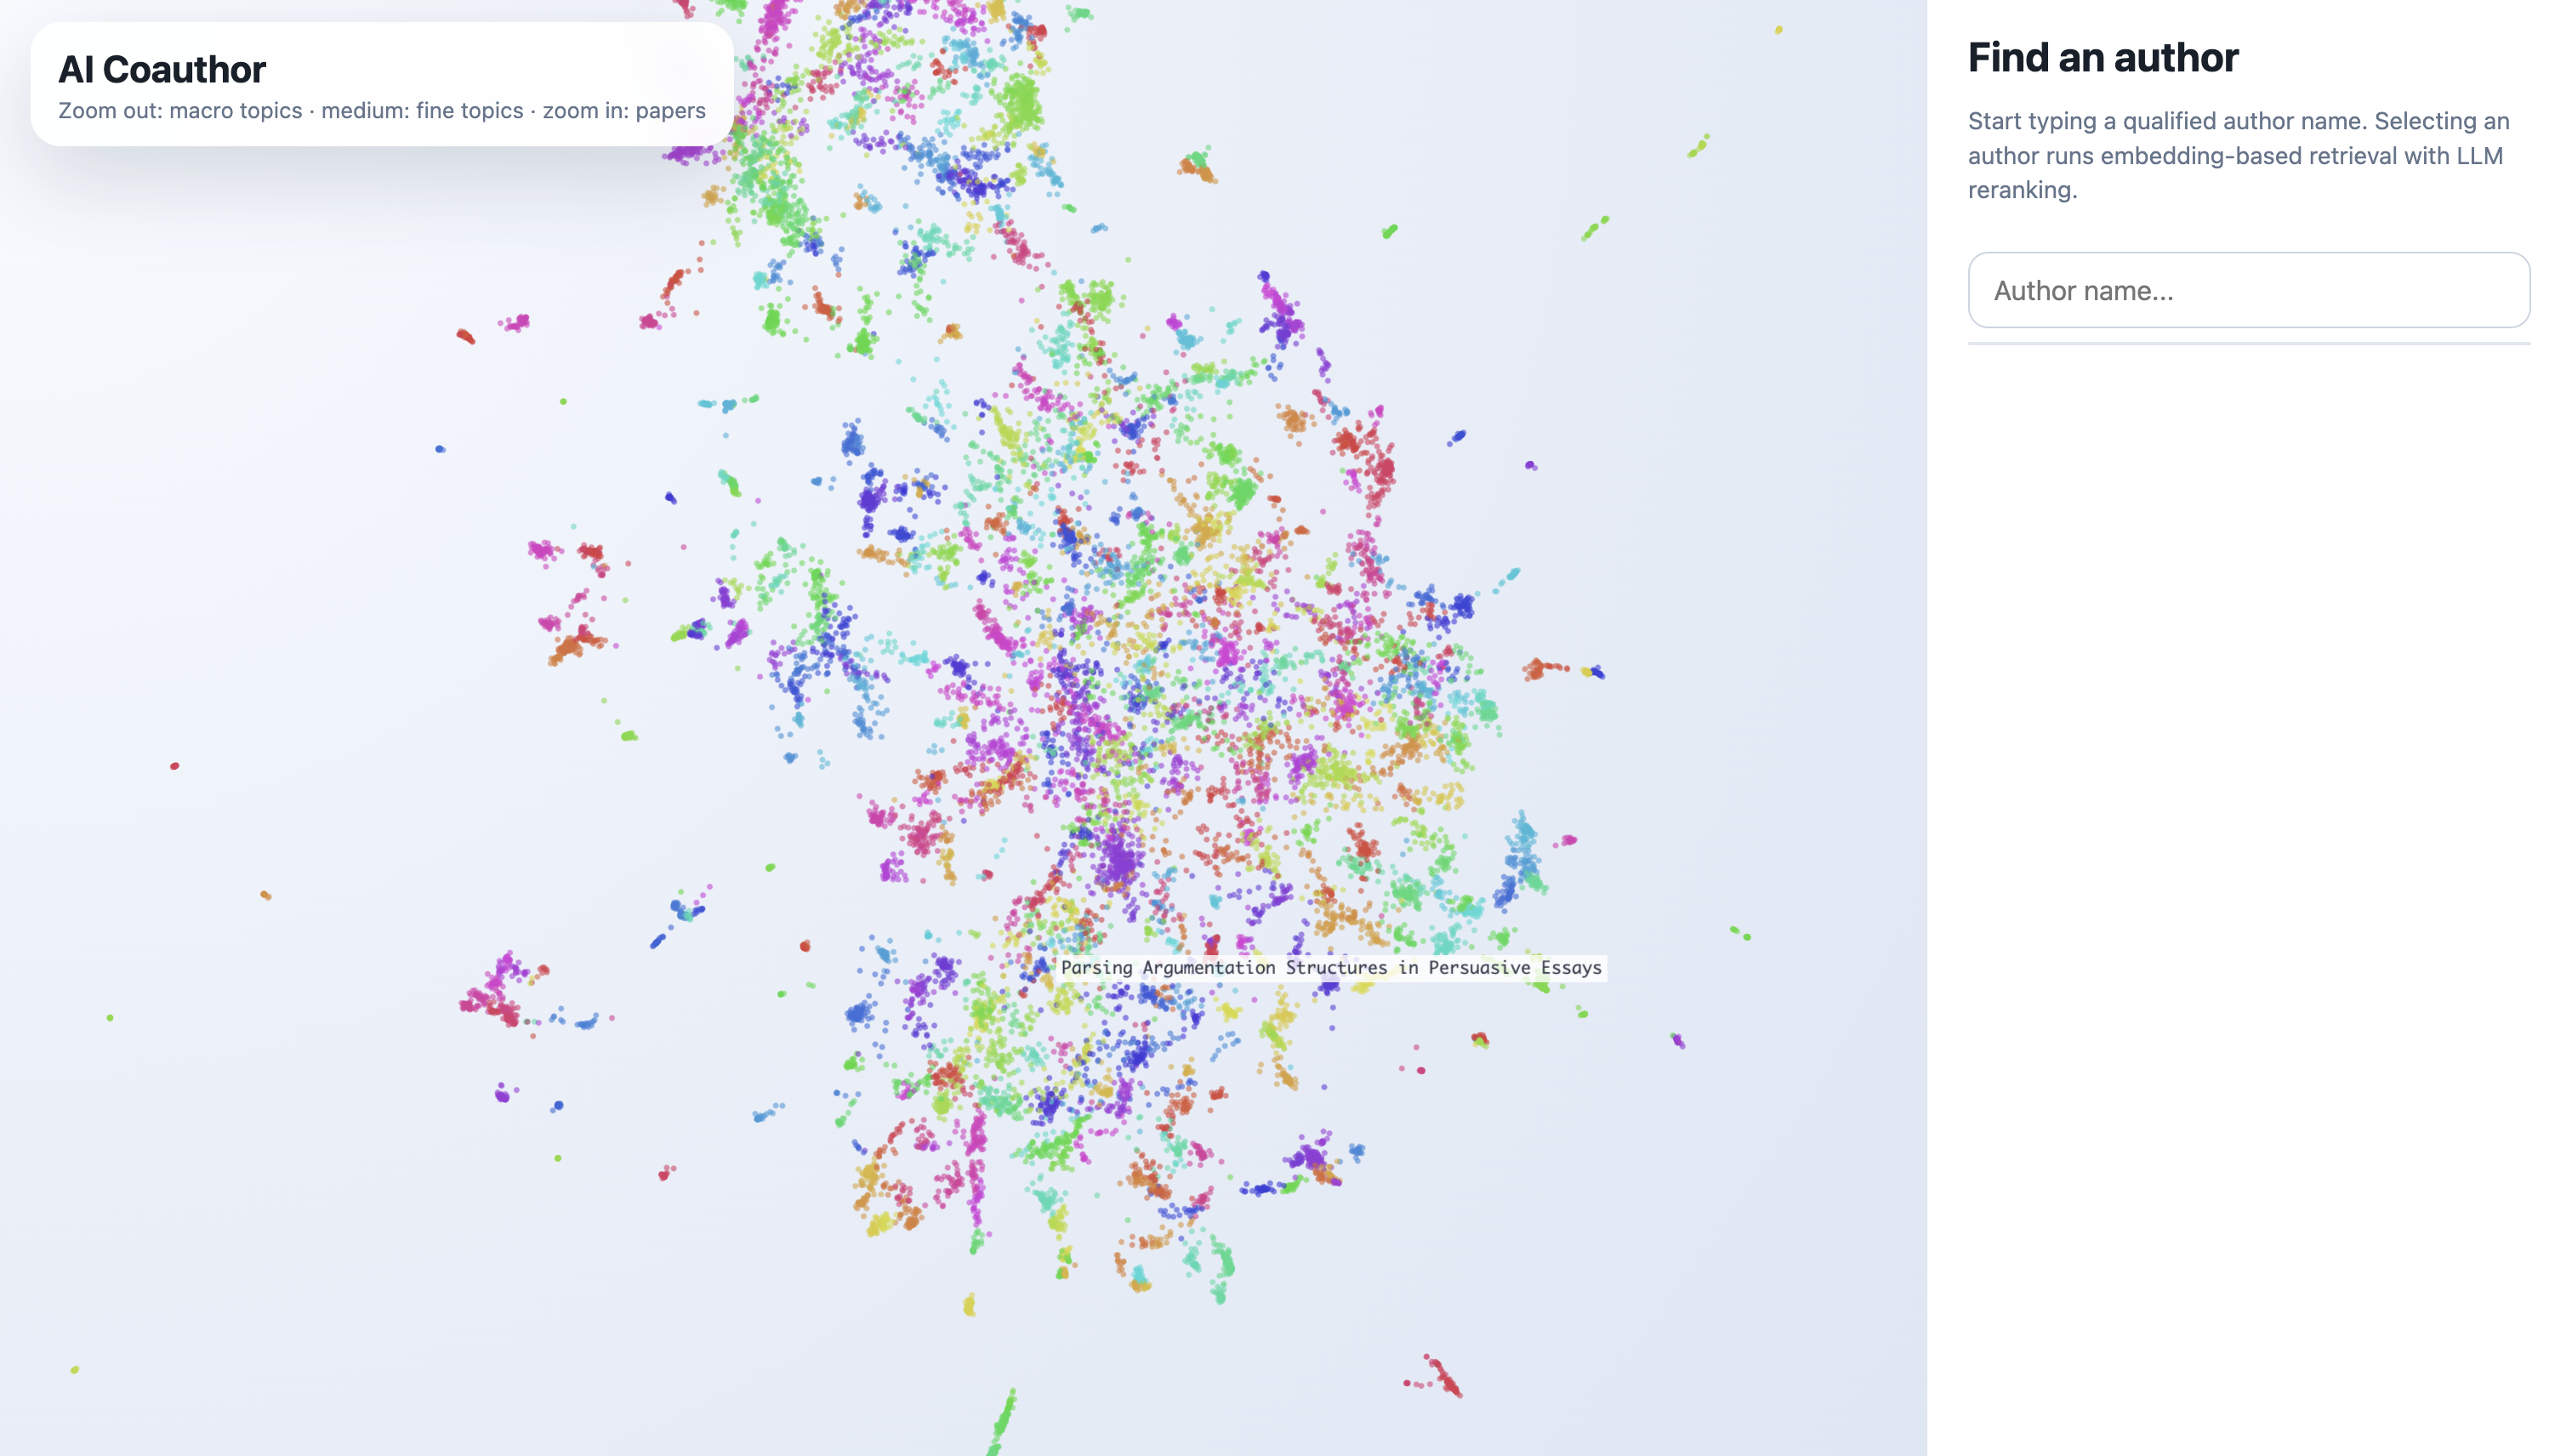
\includegraphics[width=\textwidth]{ui_map.png}
\caption{Карта научного пространства: каждая точка — статья, цвет наследуется от метакластера}
\label{fig:map}
\end{figure}

Клик по статье открывает боковую панель с деталями — заголовком, аннотацией, годом, авторами,
темой, метакластером и ссылкой на OpenAlex; поле поиска авторов поддерживает автодополнение с
транслитерацией кириллицы (рис.~\ref{fig:panel}). Выбор автора запускает пайплайн рекомендаций, и в
модальном окне показываются кандидаты с типом связи, кратким объяснением и компактными
доказательствами — попарными связями статей с короткой причиной и ссылками OpenAlex
(рис.~\ref{fig:recs}).

\begin{figure}[ht]
\centering
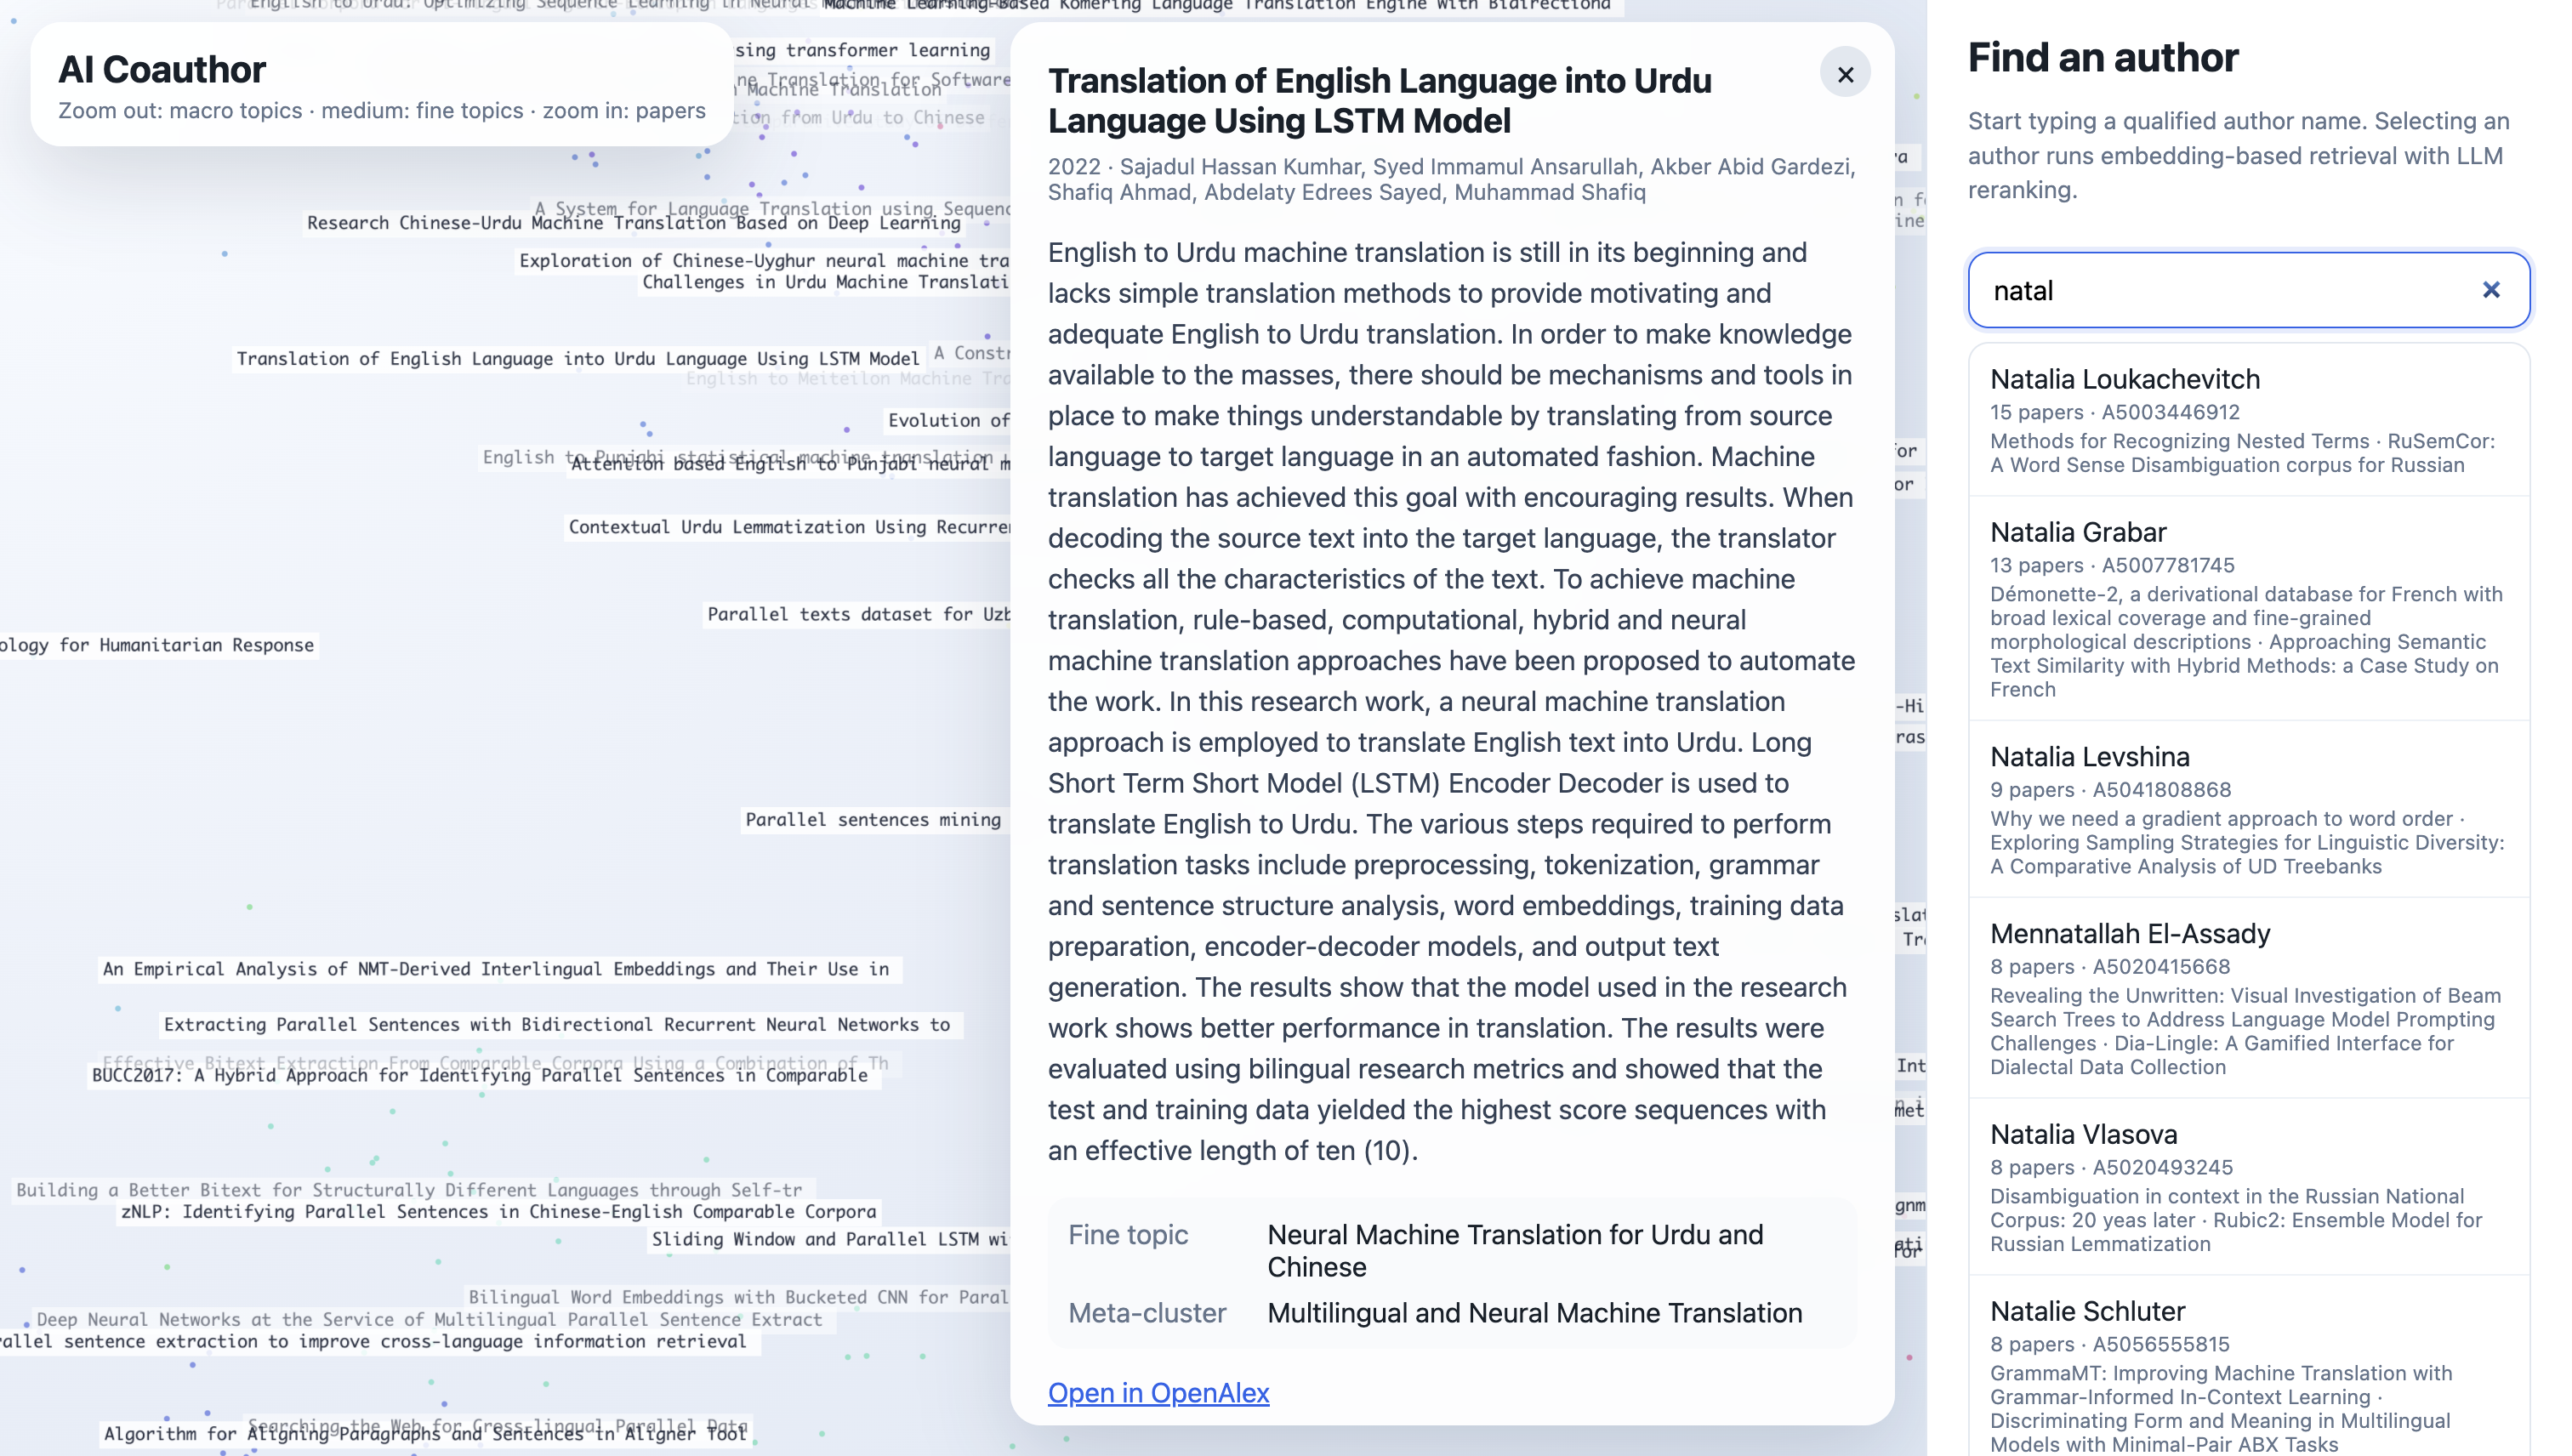
\includegraphics[width=0.95\textwidth]{ui_paper_panel.png}
\caption{Боковая панель статьи и поиск автора с автодополнением}
\label{fig:panel}
\end{figure}

\begin{figure}[ht]
\centering

\includegraphics[width=0.92\textwidth]{ui_recommendations.png}
\caption{Окно рекомендаций: кандидат, тип связи, объяснение и попарные доказательства}
\label{fig:recs}
\end{figure}

\FloatBarrier
\subsection{Выводы и результаты по главе}
\label{sec:ch2-summary}

В главе описана реализация всех подсистем. Корпус из 509\,447 статей Artificial Intelligence
представлен L2-нормализованными эмбеддингами multilingual-e5-base; конвейер в стиле BERTopic дал
979 интерпретируемых тем, объединённых в 76 метакластеров. Рекомендатель реализован в две стадии:
обучаемые Transformer- и GraphSAGE-представления автора (остаток поверх mean-бейзлайна,
coauthor InfoNCE) извлекают ближайших кандидатов, а пятиступенчатый пайплайн на языковой модели
переранжирует их и формирует объяснения с конкретными попарными доказательствами. Всё интегрировано в
веб-приложение с интерактивной картой и поиском. Количественные обоснования сделанных выборов —
сравнение кластеризации с бейзлайнами, retrieval-метрики и LLM-оценка качества — приводятся в главе~3.

\newpage
\section{Эксперименты}
\label{ch:experiments}

Все числа в этой главе взяты из реальных артефактов запусков (\code{data/}, \code{results/}).
Экспериментальный контур — корпус подполя \textbf{Artificial Intelligence} в OpenAlex.

\subsection{Датасет}
\label{sec:dataset}

Источник — OpenAlex, фильтр по подполю AI. Для retrieval отбираются \textbf{квалифицированные авторы}
($\geq 10$ публикаций, $\geq 10$ статей в истории до cutoff 2024), затем сохраняются только их статьи.

\begin{table}[ht]
\caption{Характеристики датасета}
\label{tab:dataset}
\centering
\footnotesize
\begin{tabular}{lr}
\toprule
Характеристика & Значение \\
\midrule
Статей после фильтра & 509\,447 \\
Квалифицированных авторов ($\geq 10$ статей) & 35\,954 \\
Размерность эмбеддинга статьи & 768 (multilingual-e5-base) \\
Префикс эмбеддера & \texttt{query:} + title + abstract \\
UMAP для кластеризации & $n_{\mathrm{components}} = 10$ \\
Soft membership автора $q$ & 980 (979 fine-кластеров + шум) \\
\bottomrule
\end{tabular}
\end{table}

\textbf{Разбиение для retrieval} — двухэтапное (см. \code{data/authors/dataset_meta.json}):

\begin{enumerate}
  \item \textbf{По авторам:} 80\,\% / 10\,\% / 10\,\% $\to$ train / val / test ($\mathrm{seed} = 42$).
  \item \textbf{По годам внутри каждого автора:} история — публикации $\leq 2024$, таргет —
        \textbf{новые квалифицированные coauthors} из статей $> 2024$ (не встречавшиеся в прошлой
        истории).
\end{enumerate}

\begin{table}[ht]
\caption{Разбиение примеров retrieval}
\label{tab:splits}
\centering
\footnotesize
\begin{tabular}{lrr}
\toprule
Split & Примеров & С $\geq 1$ релевантным coauthor \\
\midrule
train & 16\,210 & 7\,773 (для обучения) \\
val   & 2\,021  & 280 \\
test  & 1\,973  & 279 \\
\bottomrule
\end{tabular}
\end{table}

Порог $\geq 10$ статей выбран осознанно: при более мягком фильтре ($\geq 5$) число test-примеров
с релевантными coauthors растёт, но короткие истории (5–10 статей) делают mean-бейзлайн слишком
сильным, и относительный выигрыш Transformer снижается.

\subsection{Кластеризация: HDBSCAN и бейзлайны}
\label{sec:exp-cluster}

\subsubsection{Пайплайн оценки}

Конвейер кластеризации:
\begin{center}
\small
эмбеддинги $\to$ UMAP-10 $\to$ \{HDBSCAN | K-Means | random\}
$\to$ c-TF-IDF $\to$ MMR $\to$ LLM-метки $\to$ coherence / distinctness / quant
\end{center}

Сравниваются два варианта HDBSCAN (fine и medium) и сетка наивных бейзлайнов
\texttt{kmeans\_umap10\_k*} / \texttt{random\_umap10\_k*} на UMAP-10 с $K \in \{50, 100, 200, 400,
600, 800, 1000\}$. LLM-оценка (coherence, distinctness) запускалась для \texttt{hdbscan\_fine},
\texttt{hdbscan\_medium} и бейзлайнов K-Means при $K$, совпадающем с числом кластеров победителя
(979) и \texttt{hdbscan\_medium} (242).

Метрики в таблицах ниже \emph{независимы} — сводный взвешенный балл не используется. Когерентность
$c$ (шкала судьи 0–3) нормируется к $[0,1]$: $\hat{c} = c/3$. Остальные метрики уже лежат в $[0,1]$:
$d$ — доля дублирующих пар, $n$ — доля шума, top5 — доля корпуса в пяти крупнейших кластерах.

\subsubsection{Количественные метрики}

Источник: \code{results/summary_metrics_quant.csv}. Таблица~\ref{tab:quant-cluster} — варианты
HDBSCAN и выбранные бейзлайны (полная сетка по $K$ — в артефакте).

\begin{table}[ht]
\caption{Количественные метрики кластеризации (AI-корпус, 509\,447 статей)}
\label{tab:quant-cluster}
\centering
\footnotesize
\setlength{\tabcolsep}{3pt}
\begin{tabular}{lrrrrr}
\toprule
variant & $K$ & $e$ & size\_p50 & top5 & $n$ \\
\midrule
\textbf{hdbscan\_fine}   & \textbf{979} & 0.019 & 112   & 0.032 & \textbf{0.647} \\
hdbscan\_medium          & 242 & 0.032 & 581   & 0.253 & 0.358 \\
kmeans\_umap10\_k979     & 979 & 0.000 & 442   & 0.021 & 0.000 \\
kmeans\_umap10\_k242     & 242 & 0.000 & 1911  & 0.077 & 0.000 \\
random\_umap10\_k1000    & 1000 & 0.000 & 509   & 0.006 & 0.000 \\
\bottomrule
\end{tabular}
\end{table}

На масштабе 509\,447 статей HDBSCAN даёт много мелких тем ($K = 979$) ценой высокой доли шума
($n = 0{,}65$): значительная часть статей не попадает в плотные кластеры. K-Means и random с
фиксированным $K$ дают полное покрытие ($n = 0$) и нулевую энтропию назначений ($e = 0$) — hard
assignment без мягких вероятностей.

\subsubsection{LLM-метрики и сравнение с бейзлайнами}

Источник: \code{results/summary_metrics.csv}, \code{results/selection_report.md}.

\begin{table}[ht]
\caption{LLM-метрики кластеризации (нормированные к $[0,1]$)}
\label{tab:llm-cluster}
\centering
\footnotesize
\setlength{\tabcolsep}{3pt}
\begin{tabular}{lrrrrrr}
\toprule
variant & $K$ & $\hat{c}$ & $d$ & $e$ & top5 & $n$ \\
\midrule
\textbf{hdbscan\_fine}   & \textbf{979} & \textbf{0.934} & 0.107 & 0.019 & 0.032 & 0.647 \\
hdbscan\_medium          & 242 & 0.805 & 0.010 & 0.032 & 0.253 & 0.358 \\
kmeans\_umap10\_k979     & 979 & 0.726 & 0.260 & 0.000 & 0.021 & 0.000 \\
kmeans\_umap10\_k242     & 242 & 0.623 & 0.033 & 0.000 & 0.077 & 0.000 \\
\bottomrule
\end{tabular}
\end{table}

\begin{table}[ht]
\caption{Прирост hdbscan\_fine относительно K-Means при $K = 979$}
\label{tab:cluster-delta}
\centering
\footnotesize
\begin{tabular}{lrrr}
\toprule
Метрика & hdbscan\_fine & kmeans\_k979 & $\Delta$ (лучше $\uparrow$ / $\downarrow$) \\
\midrule
$\hat{c}$ (когерентность) & 0.934 & 0.726 & $+0.208\,\uparrow$ \\
$d$ (дубли, меньше лучше) & 0.107 & 0.260 & $-0.153\,\downarrow$ \\
top5 (меньше лучше)       & 0.032 & 0.021 & $+0.011$ \\
$n$ (шум, меньше лучше)   & 0.647 & 0.000 & $+0.647$ \\
\bottomrule
\end{tabular}
\end{table}

\textbf{Обоснование выбора \texttt{hdbscan\_fine}.} Выбор лучшего метода для наших целей неочевиден:
у каждого варианта свои сильные стороны. \texttt{hdbscan\_medium} существенно лучше по различимости
($d = 0{,}01$) и доле шума ($n = 0{,}36$), но проигрывает по когерентности ($\hat{c} = 0{,}81$
против $0{,}93$) и даёт крупные темы (медиана 581 статья). K-Means при $K = 979$ достигает
$\hat{c} = 0{,}73$, но $d = 0{,}26$ — почти четверть проверенных пар тем дублируют друг друга.

Для fine-слоя приоритет — \textbf{интерпретируемость и детализация карты}. \texttt{hdbscan\_fine}
выбран по наибольшей когерентности ($c = 2{,}80$, $\hat{c} = 0{,}93$) с явной оговоркой: доля
шума $n = 0{,}65$ высока, но это осознанный компромисс плотностной кластеризации на
неоднородном AI-корпусе — лучше честно пометить фоновые статьи шумом, чем размывать темы ради
полного покрытия.

\subsubsection{Метакластеры}

Fine-темы (\texttt{hdbscan\_fine}, $K = 979$) объединены в метакластеры по эмбеддингам
метадокументов (multilingual-e5-base, префикс \texttt{query:}). LLM-оценка — отдельные судьи
(\code{metric_meta_coherence.py}, \code{metric_meta_distinctness.py}): судья оценивает,
насколько fine-темы образуют одну \emph{широкую} исследовательскую область. Вес когерентности —
по числу статей fine-кластеров в метакластере, не по числу fine-тем.

\begin{table}[ht]
\caption{LLM-метрики метакластеризации ($K = 76$)}
\label{tab:meta-cluster}
\centering
\footnotesize
\begin{tabular}{lrrrrr}
\toprule
variant & $K$ & $\hat{c}$ & $d$ & $e$ & $n$ \\
\midrule
\textbf{meta\_hdbscan\_medium} & \textbf{76} & \textbf{0.903} & 0.000 & 0.330 & 0.114 \\
meta\_kmeans\_umap10\_k76      & 76 & 0.806 & 0.000 & 0.000 & 0.000 \\
\bottomrule
\end{tabular}
\end{table}

\textbf{Итог:} \texttt{meta\_hdbscan\_medium} — победитель по когерентности; K-Means при том же
$K = 76$ ниже ($\hat{c} = 0{,}81$). Числа meta-coherence \textbf{не сопоставимы} напрямую с
fine ($\hat{c} = 0{,}93$): другая постановка судьи и другая шкала интерпретации (широкая область
против узкой fine-темы).

\subsection{Author retrieval: семантика, граф и метакластеры}
\label{sec:exp-retrieval}

\subsubsection{Постановка и протокол оценки}

Задача — \textbf{retrieval} потенциальных coauthors: по истории автора ($\leq 2024$) найти авторов
из того же split, которые станут новыми coauthors после 2024. Этот observed-сигнал неполный:
многие хорошие рекомендации не успевают стать фактическими соавторствами в test-периоде, поэтому
observed-метрики используются как строгий нижний proxy, а LLM-оценка — как проверка смысловой
релевантности кандидатов.

\begin{itemize}
  \item \textbf{Loss:} multi-positive coauthor InfoNCE; позитивы исключены из знаменателя.
  \item \textbf{Early stopping:} val nDCG@50.
  \item \textbf{Основной онлайн-бюджет:} retrieval отдаёт $K = 10$ кандидатов, затем LLM выбирает
        3 автора для финальной рекомендации.
  \item \textbf{Сравниваемые сигналы:} mean semantic baseline, Transformer по истории статей,
        GraphSAGE по графу соавторства и комбинированный Transformer+GraphSAGE.
\end{itemize}

\subsubsection{Конфигурации моделей}

Transformer-варианты используют $d_{\mathrm{model}} = 256$, 2 слоя, 4 головы внимания, dropout 0.2,
batch\_size 64, $n_{\mathrm{negatives}} = 256$, $\tau = 0{,}05$, max\_history 20, AdamW с
$\mathrm{lr}=2\cdot10^{-4}$ и $\mathrm{weight\_decay}=0{,}05$. Для \code{author_retriever}
лучший чекпойнт выбран на epoch 7 по val nDCG@50; для \code{transformer_author_no_cluster} —
на epoch 4.

GraphSAGE-варианты используют 2 слоя, hidden\_dim 256, dropout 0.2, $n_{\mathrm{negatives}} = 256$,
$\tau = 0{,}05$, max\_history 20, AdamW с $\mathrm{lr}=10^{-3}$ и
$\mathrm{weight\_decay}=10^{-2}$. В графе 35\,954 авторских узла и 464\,752 направленных
author-author ребра. В варианте с метакластерами добавлены 76 meta-узлов и 172\,376 направленных
author-meta/meta-author рёбер. Лучшие чекпойнты по val nDCG@50: epoch 11 для
\code{graphsage_author}, epoch 60 для \code{graphsage_author_metacluster}, epoch 19 для
\code{graphsage_transformer_author}.

\subsubsection{Observed-метрики}

Источник: \code{results/retrieval/consistency/retrieval_metrics_at_k.csv} и
\code{results/retrieval/transformer_variants_metrics.csv}. Все числа в таблице~\ref{tab:retrieval-observed}
посчитаны на test при $K = 10$.

\begin{table}[ht]
\caption{Observed-метрики retrieval на test ($K = 10$)}
\label{tab:retrieval-observed}
\centering
\footnotesize
\setlength{\tabcolsep}{4pt}
\begin{tabular}{lrrrr}
\toprule
Метод & Hit@10 & MRR@10 & nDCG@10 & Recall@10 \\
\midrule
Mean embedding & 0.0172 & 0.0059 & 0.0076 & 0.0148 \\
Transformer (no cluster) & 0.0198 & 0.0071 & 0.0088 & 0.0173 \\
Transformer + fine $q$ & 0.0198 & 0.0073 & 0.0089 & 0.0168 \\
GraphSAGE & 0.0182 & 0.0074 & 0.0087 & 0.0150 \\
GraphSAGE + meta & 0.0203 & 0.0072 & 0.0087 & 0.0169 \\
\textbf{Transformer + GraphSAGE} & \textbf{0.0223} & \textbf{0.0086} & \textbf{0.0102} & \textbf{0.0186} \\
\bottomrule
\end{tabular}
\end{table}

Результат важен не абсолютным размером прироста, а сравнением источников сигнала. Mean embedding
уже силён: у всех авторов в выборке длинная история ($\geq 10$ статей), а paper embeddings хорошо
отражают тематику. Transformer без кластеров и Transformer с fine $q$ почти совпадают по Hit@10 и
nDCG@10; значит, кластерные признаки в semantic retriever не дают явного выигрыша. GraphSAGE без
метакластеров также близок к Transformer: граф прошлого соавторства содержит сильный сигнал, но он
во многом скоррелирован с семантической близостью статей. Комбинированный Transformer+GraphSAGE
показывает лучший observed nDCG@10, но разница мала на фоне разреженности target-разметки.

\subsubsection{LLM-оценка рекомендаций}

LLM-оценка запускалась на 40 test-users и top-10 кандидатах. Здесь порядок внутри top-10 не является
главной целью, потому что LLM оценивает всех 10 кандидатов и затем выбирает трёх. Поэтому в
таблице~\ref{tab:retrieval-llm} основные метрики — наличие достаточного числа релевантных
кандидатов и качество выбранной тройки.

\begin{table}[ht]
\caption{LLM-оценка retrieval (40 пользователей, $K = 10$)}
\label{tab:retrieval-llm}
\centering
\scriptsize
\setlength{\tabcolsep}{3pt}
\begin{tabular}{lrrrrr}
\toprule
Метод & Has3 $\geq 2$ & Selected3Mean & Hit $=3$ & MRR $=3$ & Has3 $=3$ \\
\midrule
Transformer + fine $q$ & 0.875 & 2.425 & 0.625 & 0.491 & 0.450 \\
GraphSAGE + meta & 0.775 & 2.367 & 0.700 & \textbf{0.541} & 0.425 \\
\textbf{Transformer + GraphSAGE} & \textbf{0.875} & \textbf{2.492} & \textbf{0.750} & 0.521 & \textbf{0.450} \\
\bottomrule
\end{tabular}
\end{table}

Has3 $\geq 2$ означает долю пользователей, для которых в top-10 есть хотя бы три кандидата с
LLM-оценкой 2 или 3. Selected3Mean — средняя LLM-оценка трёх лучших кандидатов после
переранжирования. Диагностические Hit/MRR/Has3 при score $=3$ показывают наличие очень сильных
кандидатов, но не являются основной целью системы.

GraphSAGE можно включать в работу: он показывает сопоставимое качество с Transformer и даёт
понятную проверку гипотезы о пользе графа соавторства. При этом текущие результаты не позволяют
утверждать значимый выигрыш от кластеризации в рекомендациях. Метакластерные узлы чуть меняют
observed-метрики, но paired bootstrap для метакластерного GraphSAGE против базового GraphSAGE
даёт доверительные интервалы, включающие ноль: для Hit@10
$\Delta = 0{,}0020$, 95\,\% CI $[-0{,}0025;\,0{,}0066]$, для nDCG@10
$\Delta = 0{,}0001$, 95\,\% CI $[-0{,}0022;\,0{,}0023]$. Поэтому в финальной интерпретации
кластеризация остаётся главным образом инструментом карты и интерпретации тем, а не доказанным
источником прироста retrieval.

\subsection{Выводы и результаты по главе}

В главе проведена экспериментальная проверка двух частей системы: тематической кластеризации и
recommendation pipeline. Для кластеризации HDBSCAN выбран не по одной метрике, а по совокупности
сигналов: осмысленность тем по LLM-оценке, intruder detection, различимость тем, когерентность
эмбеддингов и допустимый компромисс по доле шума. Итоговая конфигурация даёт 979 fine-тем, а
дополнительная метакластеризация объединяет их в 76 крупных направлений для навигации по карте.

Для рекомендаций сравнение mean-бейзлайна, Transformer, GraphSAGE и гибридного варианта показывает,
что семантика статей и граф соавторства дают близкие сигналы. Гибрид Transformer+GraphSAGE имеет
лучшие observed-метрики среди запущенных вариантов и лучшую LLM Selected3Mean@10, но bootstrap
для метакластерных графовых узлов не даёт значимого прироста. Поэтому основной вывод такой:
кластеризация хорошо работает как слой интерпретации и визуальной навигации, а её вклад в retrieval
на текущих данных остаётся недоказанным.


% Заключение
\newpage
\section{Заключение}

В работе разработана и реализована система AI Coauthor — комплекс для семантического анализа
научного пространства, тематической кластеризации публикаций и рекомендации потенциальных
соавторов с объяснениями на основе LLM. Система объединяет офлайн-предподсчёт эмбеддингов,
кластеризацию, построение метакластеров, обучение retrieval-моделей и онлайн-этап
LLM-переранжирования.

Эмпирическая часть построена на корпусе из 509\,447 публикаций OpenAlex по подполю Artificial
Intelligence. Статьи представлены 768-мерными эмбеддингами multilingual-e5-base. Для карты
научного пространства выбран BERTopic-style pipeline: UMAP, HDBSCAN, c-TF-IDF, MMR и
LLM-разметка тем. Итоговая структура содержит 979 fine-тем и 76 метакластеров. HDBSCAN выбран по
совокупности метрик качества тем, а не только по внутренним геометрическим критериям.

В рекомендательной части сравнивались mean-бейзлайн, Transformer-представление автора, GraphSAGE
по графу соавторства и гибрид Transformer+GraphSAGE. Финальный LLM-этап работает с top-10
кандидатами retrieval и выбирает 3 рекомендации. Качество финальной выдачи подтверждено
LLM-оценкой: LLM Selected3Mean@10 достигает 2,492 из 3, а LLM Has3@10 при score $\geq 2$ равен
0,875. Observed-метрики по будущим соавторам используются как строгий proxy retrieval, но не как
основное подтверждение релевантности рекомендаций.

Полученные результаты показывают, что граф соавторства даёт качество, сопоставимое с
Transformer-представлением автора, но явного значимого выигрыша от метакластерных узлов в retrieval
не получено. Поэтому кластеризация в текущей версии системы прежде всего полезна как слой
интерпретации: она делает карту научного пространства читаемой, даёт названия тем и связывает
рекомендации с тематической структурой корпуса. Её вклад в качество извлечения кандидатов требует
дополнительной проверки на более широкой выборке и более строгой LLM-evaluation.

Основные ограничения связаны с жёстким назначением статей в темы, искажениями 2D-проекции,
разреженностью будущих соавторств как target-разметки и тем, что в работе используются только
заголовки и аннотации, без полного текста публикаций. Направления развития — мягкое overlapping
назначение тем, использование полного текста, расширение корпуса за пределы Artificial
Intelligence и автоматизация полного воспроизводимого пайплайна.


% Библиографический список
\newpage
\printbibliography[title={Библиографический список}]
\addcontentsline{toc}{section}{Библиографический список}

% Приложения
\newpage
\appendix
\section*{Приложение А. Структура проекта}
\addcontentsline{toc}{section}{Приложение А. Структура проекта}

Ниже приведена файловая структура проекта (служебные и сгенерированные каталоги опущены).
Переиспользуемый код собран в пакете \code{src/} и разбит по доменам; запускаемые сценарии вынесены
в \code{scripts/}, а гиперпараметры — в \code{configs/}.

{\footnotesize
\begin{verbatim}
coursework/
|-- src/                      переиспользуемый код (пакеты по доменам)
|   |-- common/               конфигурация, пути, ввод-вывод, кэш LLM
|   |-- data/                 загрузка OpenAlex, сборка истории авторов
|   |-- embeddings/           векторизация статей и метадокументов (e5-base)
|   |-- clustering/
|   |   |-- paper_topics/     UMAP, HDBSCAN, бейзлайны, c-TF-IDF, MMR
|   |   \-- meta_topics/      метакластеры и UI-маппинги
|   |-- recommendation/       модель автора, обучение, retrieval-пайплайн
|   |-- llm/                  разметка тем, LLM-оценка рекомендаций
|   |-- evaluation/           метрики кластеризации, retrieval, покрытия
|   \-- web/                  FastAPI backend + Deck.gl frontend
|-- scripts/                  запускаемые сценарии run_*.py
|-- configs/                  YAML-снимки гиперпараметров
|-- data/                     сырые и промежуточные артефакты
|-- models/                   веса обученных моделей
|-- results/                  метрики, отчёты, графики
\-- docs/                     проектная документация
\end{verbatim}
}


\end{document}
